% GAUSSIAN FITTING
First of all, we consider the problem of fitting a Gaussian distribution \(\mathcal{N}(y_i \cond \mu,\sigma^2)\) to random realizations \(y_i\) with \(i = 1,\ldots,\dimData\).
The goal is to estimate the unknown mean \(\mu\) whereas the standard deviation \(\sigma\) is assumed to be already known.
Given a Gaussian prior, this one-dimensional normal model with known variance exhibits a Gaussian posterior density.
Moreover, a closed-form expression for the model evidence can be derived.
Since this offers the possibility of comparing the SLE results with analytical solutions, this simple statistical model is used as a first SLE testbed.
Let the data \(\bm{y} = (y_1,\ldots,y_\dimData)^\top\) be comprised of \(\dimData\) independent samples from the normal distribution.
For the observational model one may then write
\begin{equation} \label{eq:JCP:Conjugate:Data}
  \bm{Y} \cond \mu \sim \prod\limits_{i=1}^\dimData \mathcal{N}(y_i \cond \mu,\sigma^2), \quad \text{with known} \;\, \sigma^2.
\end{equation}
% POSTERIOR DISTRIBUTION
Consequently, the likelihood function can be simply written as \(\mathcal{L}(\mu) = \prod_{i=1}^{\dimData} \mathcal{N}(y_i \cond \mu,\sigma^2)\).
A Bayesian prior distribution \(\pi(\mu)\) captures the epistemic uncertainty of the true value of \(\mu\) before the data analysis.
For the posterior distribution, that aggregates the information about the unknown after the data have been analyzed, one then has \(\pi(\mu \cond \bm{y}) = \scale^{-1} \mathcal{L}(\mu) \pi(\mu)\).
\par % CONJUGATE ANALYSIS
The conjugate prior for the data model in \cref{eq:JCP:Conjugate:Data} is a Gaussian \(\pi(\mu) = \mathcal{N}(\mu \cond \mu_0,\sigma_0^2)\).
Its mean \(\mu_0 = \mathds{E}[\mu]\) and variance \(\sigma_0^2 = \mathrm{Var}[\mu]\) have to be conveniently specified by the experimenter and data analyst.
This prior choice ensures that the posterior is a Gaussian \(\pi(\mu \cond \bm{y}) = \mathcal{N}(\mu \cond \mu_\dimData,\sigma_\dimData^2)\)
whose parameters \(\mu_\dimData = \mathds{E}[\mu \cond \bm{y}]\) and \(\sigma_\dimData^2 = \mathrm{Var}[\mu \cond \bm{y}]\) are easily found as
\begin{equation} \label{eq:JCP:Conjugate:Posterior}
  \mu_\dimData = \left( \frac{1}{\sigma_0^2} + \frac{\dimData}{\sigma^2} \right)^{-1} \left( \frac{\mu_0}{\sigma_0^2} + \frac{\dimData \overline{y}}{\sigma^2} \right),
  \quad \sigma_\dimData^2 = \left( \frac{1}{\sigma_0^2} + \frac{\dimData}{\sigma^2} \right)^{-1}.
\end{equation}
Here, \(\overline{y} = N^{-1} \sum_{i=1}^N y_i\) is the empirical sample mean of the data.
% MODEL EVIDENCE
Likewise, an explicit expression for the model evidence
\(\scale = \int_{\mathds{R}} (\prod_{i=1}^\dimData \mathcal{N}(y_i \cond \mu, \sigma^2)) \, \mathcal{N}(\mu \cond \mu_0,\sigma_0^2) \, \mathrm{d} \mu\) can be derived.
Let \(\overline{y^2} = N^{-1} \sum_{i=1}^N y_i^2\) denote the sample mean of the squared observations.
A straightforward calculation based on simple algebra and a Gaussian integral then yields
\begin{equation} \label{eq:JCP:Conjugate:ModelEvidence}
  \scale = \sigma_0^{-1} \left( \sigma \sqrt{2 \pi} \right)^{-\dimData} \left( \frac{1}{\sigma_0^2} + \frac{\dimData}{\sigma^2} \right)^{-1/2}
  \exp \left( - \frac{1}{2} \left( \frac{\mu_0^2}{\sigma_0^2} + \frac{\dimData \overline{y^2}}{\sigma^2}
  - \left( \frac{1}{\sigma_0^2} + \frac{\dimData}{\sigma^2} \right)^{-1} \left( \frac{\mu_0}{\sigma_0^2} + \frac{\dimData \overline{y}}{\sigma^2} \right)^2 \right) \right).
\end{equation}
\par % EXPERIMENTAL SETUP
For the following computer experiment, the parameters of the data distribution in \cref{eq:JCP:Conjugate:Data} are specified as \(\mu = 10\) and \(\sigma = 5\), respectively.
In the course of the procedure only the mean is treated as an unknown, whereas the standard deviation is assumed to be known.
We consider a situation where \(\dimData = 10\) samples are randomly drawn from the data distribution.
For the numerical experiment, the pseudo-random numbers \(\bm{y} = (8.78,4.05,12.58,3.60,11.05,8.70,20.80,1.23,19.36,12.07)^\top\) are used as synthetic data.
The prior distribution is set to be a Gaussian \(\pi(\mu) = \mathcal{N}(\mu \cond \mu_0,\sigma_0^2)\) with \(\mu_0 = 11.5\) and \(\sigma_0 = 1.5\).

\subsubsection{Posterior density}
% LIKELIHOOD EXPANSION
In order to better understand the principles of spectral Bayesian inference we now proceed as follows.
Spectral expansions \(\hat{\mathcal{L}}_p\) of the likelihood function \(\mathcal{L}\) defined above are computed and compared
for experimental designs of varying size \(K\) and polynomial terms of varying degree \(p\).
Hermite polynomials are used in combination with an appropriate linear transformation to standardized variables
\(\xi_\mu \in \mathds{R}\) with a Gaussian weight function \(\mathcal{N}(\xi_\mu \cond 0,1)\).
Accordingly, the unknown can be represented as \(\mu = \mu_0 + \sigma_0 \xi_\mu\).
The experimental designs are one-dimensional Sobol sequences that are appropriately transformed.
\par % SLE CONVERGENCE
First the convergence behavior and the accuracy of the likelihood approximation are analyzed.
For a rich experimental design with \(K = 5 \times 10^4\), SLEs are computed for an increasing order up to \(p = 20\).
The normalized empirical error \(\epsilon_{\mathrm{Emp}}\) and the normalized LOO error \(\epsilon_{\mathrm{LOO}}\) are monitored over these computations.
While the former can be directly computed according to its definition, the computation of the latter relies on the reformulation in \cref{eq:JCP:PCE:SimpleLOO}.
This serves the purpose of assessing the prediction accuracy of the computed SLE as a function of the degree \(p\).
The results are plotted in \cref{fig:JCP:Conjugate:ConvSLE}.
It can be seen how the error estimates approach zero, i.e.\ the SLE converges to the likelihood function.
For \(p = 20\) the empirical error amounts to \(\epsilon_{\mathrm{Emp}} = 1.05 \times 10^{-12}\) and the LOO amounts to \(\epsilon_{\mathrm{LOO}} = 1.82 \times 10^{-10}\).
These small error magnitudes show that the likelihood function \(\mathcal{L}\) can be indeed spectrally expanded in a Hermite basis.
% FIGURE: SLE CONVERGENCE
\begin{figure}[htbp]
  \centering
  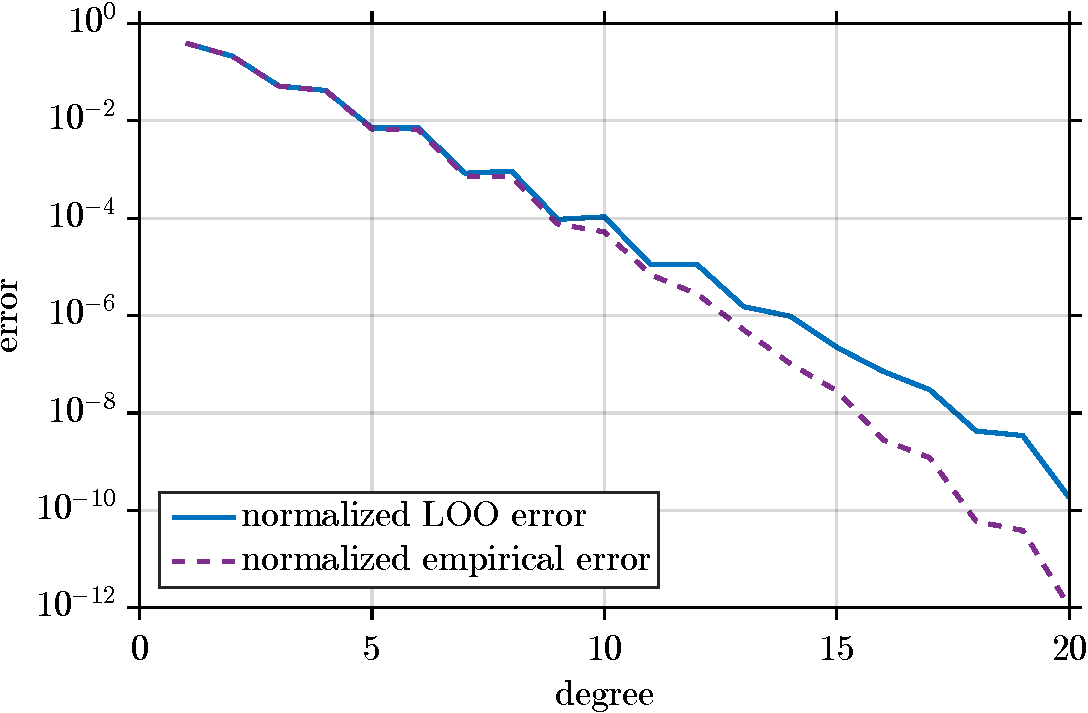
\includegraphics[height=\JCPfigHeight]{fig_JCP_Norm1D_ConvSLE}
  \caption[1D normal fitting: Convergence of the SLE]{1D normal fitting: Convergence of the SLE.}
  \label{fig:JCP:Conjugate:ConvSLE}
\end{figure}
\par % LIKELIHOOD FUNCTION
The functional likelihood approximation \(\hat{\mathcal{L}}_p\) provided by the most accurate SLE with \(p = 20\) is visualized in \cref{fig:JCP:Conjugate:Like}.
Moreover, the plot shows a low-order SLE with \(p = 5\) and \(K = 1 \times 10^2\) for which the error estimates
\(\epsilon_{\mathrm{Emp}} = 2.61 \times 10^{-4}\) and \(\epsilon_{\mathrm{LOO}} = 8.41 \times 10^{-4}\) are obtained.
For the sake of comparison the exact likelihood function \(\mathcal{L}\) is shown as well.
It can be seen that the SLEs are able to accurately represent the likelihood around its peak,
i.e.\ roughly speaking in the interval \(\mu \in [8,15]\) for \(p = 5\) and in \(\mu \in [5,18]\) for \(p = 20\).
Note that these regions accumulate the largest proportions of the total prior probability mass.
Outside of these ranges, however, the SLEs \(\hat{\mathcal{L}}_p\) start strongly deviating from \(\mathcal{L}\) and taking on negative values.
These phenomena can be attributed to an imperfect polynomial cancellation of the finite series approximation of the likelihood
in the regions of the parameter space that are only sparsely covered by the experimental design.
Indeed, for unbounded parameter spaces it is clearly hopeless to achieve a global net cancellation of a finite polynomial expansion
that is necessary in order to emulate the vanishing behavior of the likelihood far from its peaks.
The extent to which this impacts on the approximation of the posterior density and its first moments is investigated next.
\par % POSTERIOR DENSITY
Expanding the likelihood function is only a means to the end of surrogating the posterior density.
Approximations of the posterior density \(\pi(\mu \cond \bm{y}) \approx \coeffL_0^{-1} \hat{\mathcal{L}}_p(\mu) \pi(\mu)\)
are computed from the SLEs with \(p = 5\) and \(p = 20\) through \cref{eq:JCP:SLE:Posterior,eq:JCP:SLE:ScaleFactor}.
The results are plotted in \cref{fig:JCP:Conjugate:Post}.
In addition to the SLE approximations, the prior density \(\pi(\mu) = \mathcal{N}(\mu \cond \mu_0,\sigma_0^2)\) and the exact solution
\(\pi(\mu \cond \bm{y}) = \mathcal{N}(\mu \cond \mu_\dimData,\sigma_\dimData^2)\) from a conjugate analysis based on \cref{eq:JCP:Conjugate:Posterior} are shown.
The posterior surrogate for \(p = 5\) shows minor deviations from the the analytical result,
while the approximation for \(p = 20\) perfectly matches the true density.
% EXPONENTIAL DECAY
It is noted that the discrepancies between \(\hat{\mathcal{L}}_p\) and \(\mathcal{L}\) shown in \cref{fig:JCP:Conjugate:Like} are attenuated.
The underlying reason is that for large enough \(\lvert \mu \rvert \rightarrow \infty\) the exponential decay of the Gaussian prior \(\pi(\mu) \propto \exp(-(\mu-\mu_0)^2)\)
dominates the polynomial increase of \(\hat{\mathcal{L}}_p(\mu) = \sum_{\alpha=0}^p \coeffL_{\alpha} \basis_{\alpha}(\mu)\) in the sense that \(\hat{\mathcal{L}}_p(\mu) \pi(\mu) \rightarrow 0\).
This absorbs the effects of the SLE approximation that is increasingly inadequate for large values of \(\lvert \mu \rvert\).
In this sense, the prior reference density guards the posterior surrogate against the inadequacies of the SLE.
Therefore, the posterior emulation may very well be more accurate than the SLE approximation of the likelihood.
% FIGURES: LIKELIHOOD & POSTERIOR
\begin{figure}[htbp]
  \begin{minipage}[b]{\JCPsubWidth}
    \centering
    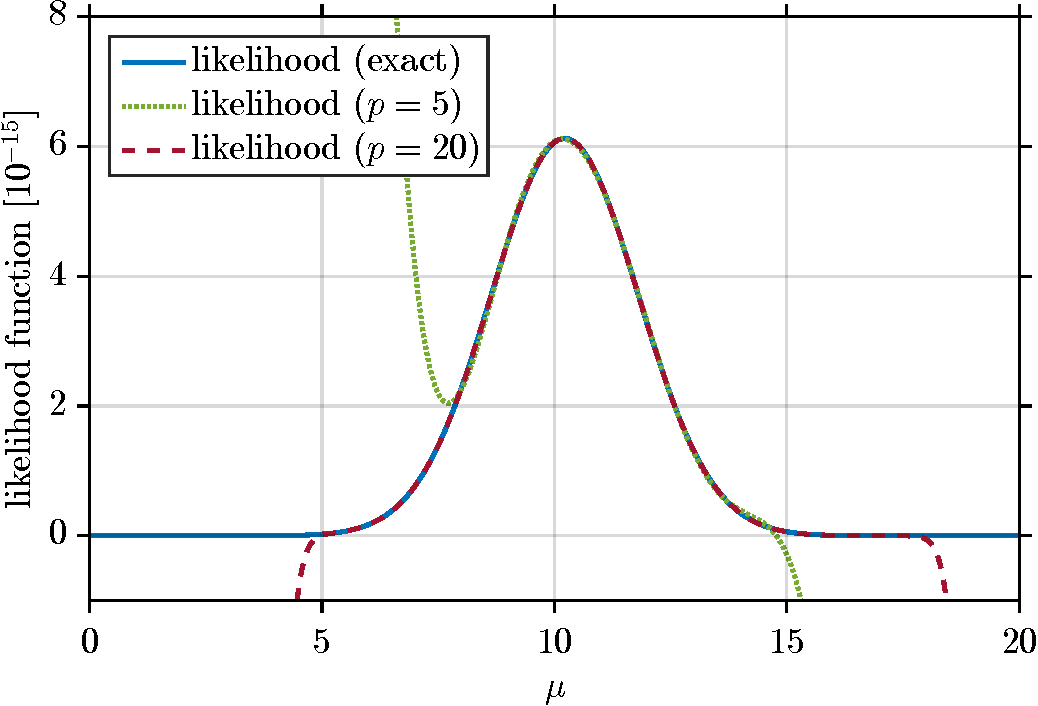
\includegraphics[height=\JCPfigHeight]{fig_JCP_Norm1D_Like}
    \caption[1D normal fitting: Likelihood function]{1D normal fitting: Likelihood function.}
    \label{fig:JCP:Conjugate:Like}
  \end{minipage}%
  \hfill%
  \begin{minipage}[b]{\JCPsubWidth}
    \centering
    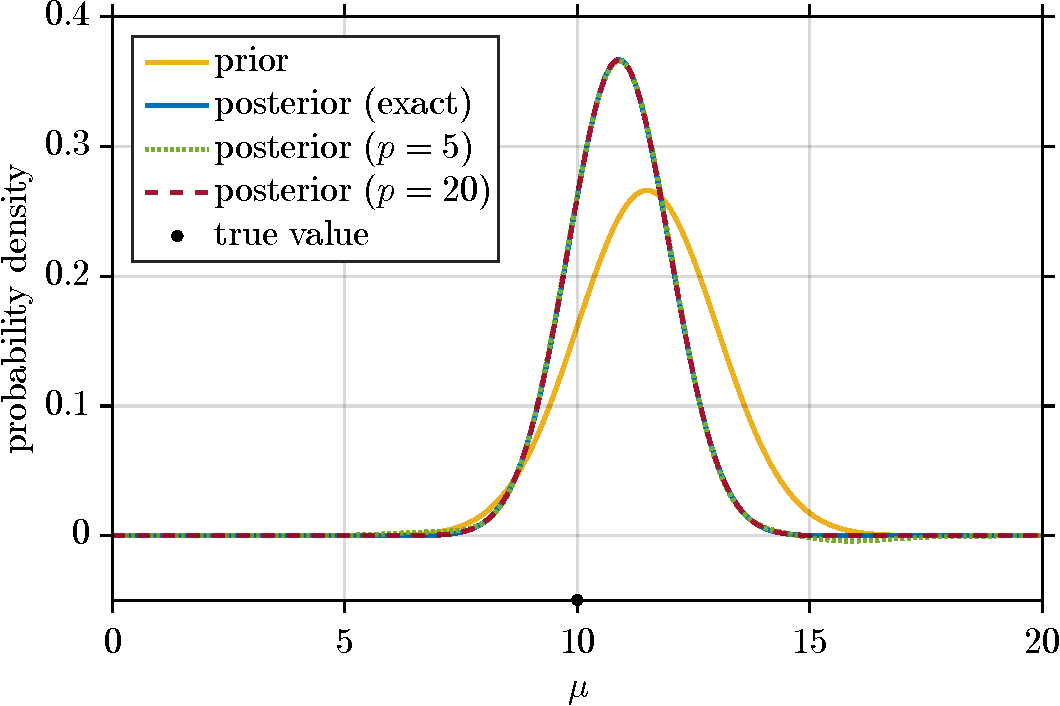
\includegraphics[height=\JCPfigHeight]{fig_JCP_Norm1D_Post}
    \caption[1D normal fitting: Posterior density]{1D normal fitting: Posterior density.}
    \label{fig:JCP:Conjugate:Post}
  \end{minipage}%
\end{figure}

\subsubsection{Quantities of interest}
% STATISTICAL QUANTITIES OF INTEREST
Commonly one employs posterior means as parameter estimates and posterior standard deviations as measures of the estimation uncertainty.
In order to investigate how well one can approximate the model evidence together with these meaningful quantities in spectral Bayesian inference,
SLEs are computed for experimental designs of varying size \(K\) and for a selection of expansion orders \(p\).
The corresponding SLE-based approximations of the model evidence \(\scale\), the posterior mean \(\mu_\dimData\) and the standard deviation \(\sigma_\dimData\)
are then computed from \cref{eq:JCP:SLE:ScaleFactor,eq:JCP:SLE:PosteriorMargMean,eq:JCP:SLE:PosteriorMargVariance}.
Note that the effects of the transformation to standard variables have to be appropriately taken care of at this place.
This happens via \cref{eq:JCP:PCE:IntegrationBySubstitution}.
The SLE approximations can then be compared to the analytical solutions that are obtained from the conjugate analysis in \cref{eq:JCP:Conjugate:Posterior,eq:JCP:Conjugate:ModelEvidence}.
In \cref{tab:JCP:Conjugate:StatisticalQuantities} the results of this procedure are summarized.
Note that all the SLE estimates attain admissible values, e.g.\ the model evidence is non-negative.
Furthermore, it is noticed that \(\scale\), \(\mu_\dimData\) and \(\sigma_\dimData\) can be recovered with high accuracy even for very scarce experimental designs and low-order SLEs,
say for \(K = 1 \times 10^3\) and \(p = 10\).
It is concluded that, in some sense, the accurate estimation of the model evidence and the first posterior moments
require significantly less computational effort than the accurate estimation of the posterior density.
% TABLE: STATISTICAL QUANTITIES
\begin{table}[htbp]
  \caption[1D normal fitting: Statistical quantities]{1D normal fitting: Statistical quantities.}
  \label{tab:JCP:Conjugate:StatisticalQuantities}
  \centering
  \begin{tabular}{ccccccc}
    \toprule
    & \(K\) & \(p\) & \(\epsilon_{\mathrm{LOO}}\) & \(\scale\) \([10^{-15}]\) & \(\mu_\dimData\) & \(\sigma_\dimData\) \\
    \midrule
    \multirow{6}{*}{\rotatebox[origin=c]{90}{SLE}}
    & \(1 \times 10^2\) &  \(5\) & \(8.41 \times 10^{-4}\) & \(3.71\) & \(10.85\) & \(0.92\) \\
    & \(5 \times 10^2\) &  \(8\) & \(2.49 \times 10^{-4}\) & \(3.75\) & \(10.91\) & \(1.14\) \\
    & \(1 \times 10^3\) & \(10\) & \(2.58 \times 10^{-5}\) & \(3.74\) & \(10.90\) & \(1.07\) \\
    & \(5 \times 10^3\) & \(12\) & \(8.21 \times 10^{-6}\) & \(3.74\) & \(10.89\) & \(1.09\) \\
    & \(1 \times 10^4\) & \(15\) & \(3.84 \times 10^{-7}\) & \(3.74\) & \(10.89\) & \(1.09\) \\
    & \(5 \times 10^4\) & \(20\) & \(\phantom{^{1}}1.82 \times 10^{-10}\) & \(3.74\) & \(10.89\) & \(1.09\) \\
    \midrule
    \multicolumn{4}{c}{Exact results}                      & \(3.74\) & \(10.89\) & \(1.09\) \\
    \bottomrule
  \end{tabular}
\end{table}